\section{Auswertung}
%
\subsubsection*{Verstärkerschaltung mit einem Transistor in Emitterschaltung}
%
Um einen Vergleich von $I_{\text{C}}$ während des Experiments mit dem zuvor berechneten, theoretischen Wert anzustellen, muss $I_{\text{C}}$ über die mit dem Multimeter bestimmte $U_{\text{C}}$ bestimmt werden:
%
\begin{align}
    \label{eq:ICausUC}
    \begin{split}
        I_C &= \frac{U_C}{R_C}
    \end{split}
    \\
    \label{eq:FehlerICausUC}
    \begin{split}
        \Delta I_C &= \sqrt{ \left ( \frac{1}{R_C} \cdot \Delta U_C \right ) ^2 + \left ( - \frac{U_C}{{R_C}^2} \cdot \Delta U_C \right ) ^2 }
    \end{split}
\end{align}
%
Die Verstärkung $V_U$ berechnet sich aus dem Quotienten von $U_{\text{SS}}$ des Ausgangssignals zu $U_{\text{SS}}$ des Eingangssignals.
Der Frequenzgang wird geplottet und ist in Abbildung \ref{fig:FrequenzgangEmitterschaltung} dargestellt.
Die untere Grenzfrequenz wird über eine Horizontale beim $\nicefrac{1}{\sqrt{2}}$-fachen des Plateaus ermittelt.
Die Vergleiche zwischen den experimentell bestimmten Werten und den Theoriewerten sind in Tabelle \ref{tab:VergleichExpTheo} aufgeführt.
%
\par
%
Auf eine detailliertere Angabe von Formeln zur Berechnung der einzelnen Größen und Messunsicherheiten wird an dieser Stelle verzichtet.
%
\par
%
\minipage{\linewidth}
    \begin{center}
        \captionsetup{type=figure}
        \begin{adjustbox}{max width=\linewidth, keepaspectratio}
            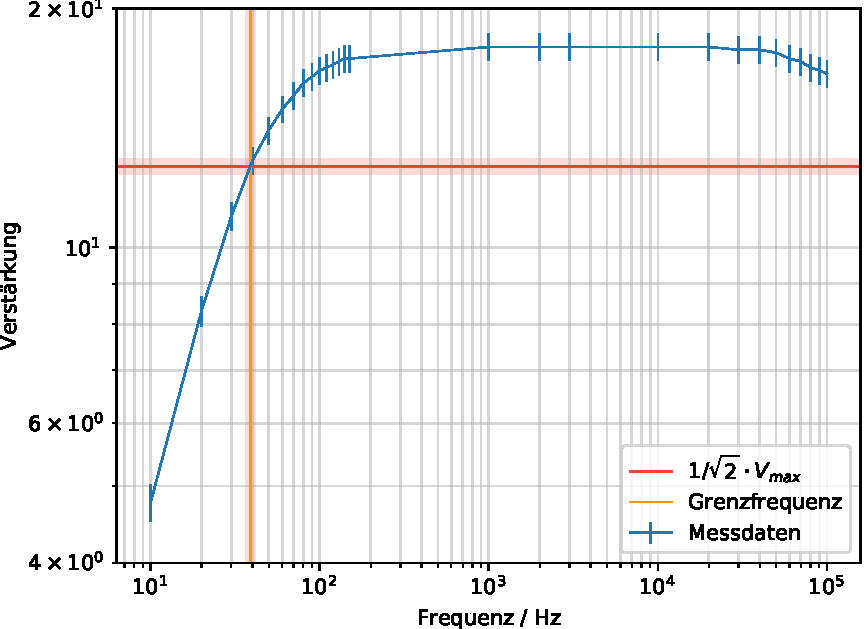
\includegraphics[]{pdf/FrequenzgangEmitterschaltung}
        \end{adjustbox}
        \captionof{figure}{Frequenzgang der Emitterschaltung}
        \label{fig:FrequenzgangEmitterschaltung}
    \end{center}
\endminipage
%
\subsubsection*{Verstärkerschaltung mit einem Transistor in Kollektorschaltung}
%
Falls im Folgenden nicht weiter beschrieben, finden die Berechnungen analog der Auswertung zum vorherigen Versuchsteil statt.
Für die Berechnung der Kabellänge wird eine Ausbreitungsgeschwindigkeit von $v = \nicefrac{2}{3} \cdot c$ angenommen, wobei $c$ die Lichtgeschwindigkeit beschreibt mit $c = \SI{299800}{\kilo\meter\per\second}$ \cite{Anleitung}.
Die Länge $L$ des Kabels berechnet sich mit:
%
\begin{align}
    \label{eq:Kabellaenge}
    \begin{split}
        L &= v \cdot t
    \end{split}
    \\
    \label{eq:FehlerKabellaenge}
    \begin{split}
        \Delta L &= v \cdot \Delta t
    \end{split}
\end{align}
%
Der Frequenzgang ist in Abbildung \ref{fig:FrequenzgangKollektorschaltung} dargestellt.
Die Vergleiche zwischen den experimentell bestimmten Werten und den Theoriewerten sind in Tabelle \ref{tab:VergleichExpTheo} aufgeführt.
%
\par
%
\minipage{\linewidth}
    \begin{center}
        \captionsetup{type=figure}
        \begin{adjustbox}{max width=\linewidth, keepaspectratio}
            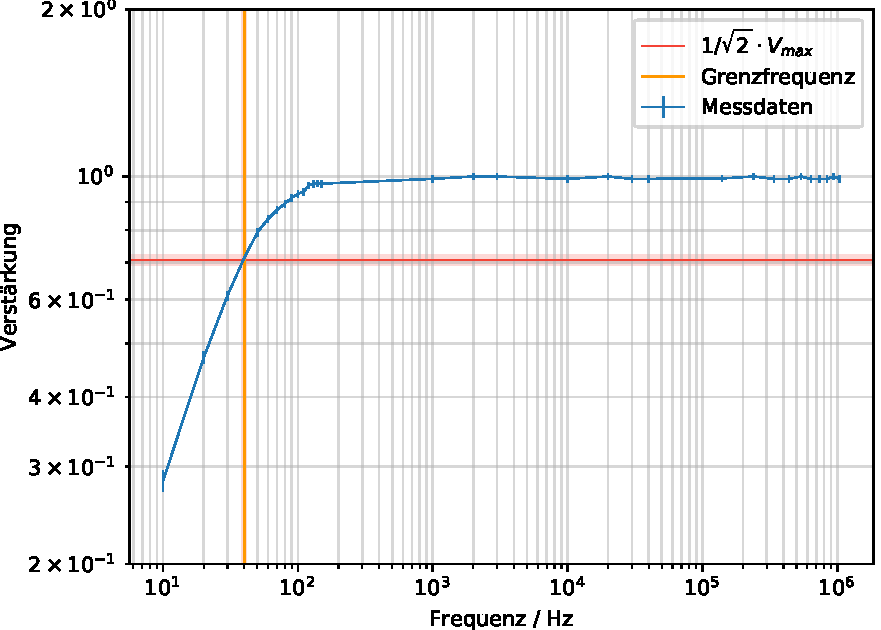
\includegraphics[]{pdf/FrequenzgangKollektorschaltung}
        \end{adjustbox}
        \captionof{figure}{Frequenzgang der Kollektorschaltung}
        \label{fig:FrequenzgangKollektorschaltung}
    \end{center}
\endminipage
%
\subsubsection*{Vergleichstabelle}
%
\minipage{\linewidth}
    \begin{center}
        \captionsetup{type=table}
        \begin{adjustbox}{max width=\linewidth, keepaspectratio}
            \begin{tabular}{lllll}
            \toprule
            Versuchsteil       & Größe             & Experimentell & Theoriewert & Abweichung \\
            \midrule
            Emitterschaltung   & $U_{\text{CE}}$   & \SI{7,85 \pm 0,05}{\volt}           & \SI{7,87 \pm 0,07}{\volt}        & \SI{0,24}{\sigma} \\
            ~                  & $U_{\text{BE}}$   & \SI{0,628 \pm 0,005}{\volt}         & \SI{0,66 \pm 0,08}{\volt}        & \SI{0,4}{\sigma}  \\
            ~                  & $U_{\text{C}}$    & \SI{6,82 \pm 0,05}{\volt}           & \SI{6,80 \pm 0,07}{\volt}        & \SI{0,23}{\sigma} \\
            ~                  & $U_{R_1}$         & \SI{14,03 \pm 0,05}{\volt}          & \SI{14,01 \pm 0,08}{\volt}       & \SI{0,21}{\sigma} \\
            ~                  & $U_{R_2}$         & \SI{0,958 \pm 0,005}{\volt}         & \SI{0,99 \pm 0,08}{\volt}        & \SI{0,4}{\sigma}  \\
            ~                  & $I_{\text{C}}$    & \SI{0,958 \pm 0,005}{\milli\ampere} & \SI{1}{\milli\ampere}            & \SI{0,25}{\sigma} \\
            ~                  & $V_U$             & \SI{17,9 \pm 0,7}{}                 & \SI{20,61 \pm 0,29}{}            & \SI{2,7}{\sigma}  \\
            ~                  & $f_{\text{uG}}$   & \SI{39 \pm 2}{\hertz}               & \SI{36 \pm 6}{\hertz}            & \SI{0,5}{\sigma}  \\
            ~                  & $R_{\text{Ein}}$  & \SI{45,4 \pm 1,0}{\kilo\ohm}        & \SI{44 \pm 6}{\kilo\ohm}         & \SI{0,16}{\sigma} \\
            ~                  & $R_{\text{Aus}}$  & \SI{5,8 \pm 1,0}{\kilo\ohm}         & \SI{6,80 \pm 0,07}{\kilo\ohm}    & \SI{1}{\sigma}    \\
            Kollektorschaltung & $U_{\text{E}}$    & \SI{7,56 \pm 0,05}{\volt}           & \SI{7,52 \pm 0,08}{\volt}        & \SI{0,4}{\sigma}  \\
            ~                  & $U_{\text{BE}}$   & \SI{0,660 \pm 0,005}{\volt}         & \SI{0,66 \pm 0,08}{\volt}        & \SI{0,01}{\sigma} \\
            ~                  & $U_{R_1}$         & \SI{6,70 \pm 0,05}{\volt}           & \SI{6,82 \pm 0,11}{\volt}        & \SI{1,0}{\sigma}  \\
            ~                  & $U_{R_2}$         & \SI{8,25 \pm 0,05}{\volt}           & \SI{8,18 \pm 0,11}{\volt}        & \SI{0,6}{\sigma}  \\
            ~                  & $I_{\text{E}}$    & \SI{16,09 \pm 0,19}{\milli\ampere}  & \SI{15,9 \pm 0,1}{\milli\ampere} & \SI{1,1}{\sigma}  \\
            ~                  & $V_U$             & \SI{0,99 \pm 0,03}{}                & \SI{0,92 \pm 0,04}{}             & \SI{1,1}{\sigma}  \\
            ~                  & $f_{\text{uG}}$   & \SI{40 \pm 1}{\hertz}               & \SI{41 \pm 5}{\hertz}            & \SI{0,2}{\sigma}  \\
            ~                  & Kabellänge $L$    & \SI{20,0 \pm 0,4}{\meter}           & \SI{20}{\meter}                  & \SI{0,07}{\sigma} \\
            ~                  & Kabelimpedanz $R$ & \SI{70 \pm 20}{\ohm}                & \SI{50}{\ohm}                    & \SI{1}{\sigma}    \\
            \bottomrule
            \end{tabular}
        \end{adjustbox}
        \captionof{table}{Vergleich der experimentell bestimmten Werte mit den Theoriewerten}
        \label{tab:VergleichExpTheo}
    \end{center}
\endminipage
